\section{Diagramme objet-interaction (4 points)}\label{doi}

Pour chaque diagramme objet-interaction, expliquer quelle est la situation décrite.

\begin{multicols}{2}
	\begin{questions}
		\question	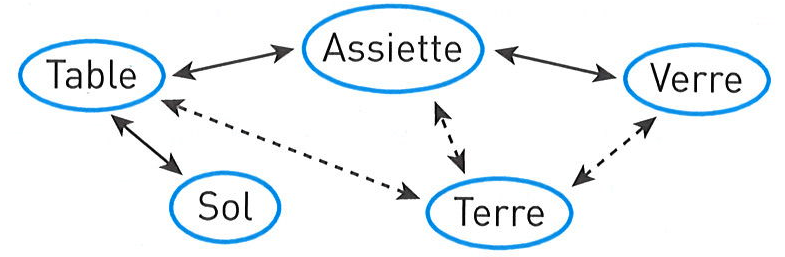
\includegraphics[scale=0.35]{doi1}
		
		\begin{solution}
			Une table posée sur le sol. Une assiette sur cette table avec un verre dedans.
		\end{solution}
		
		\question 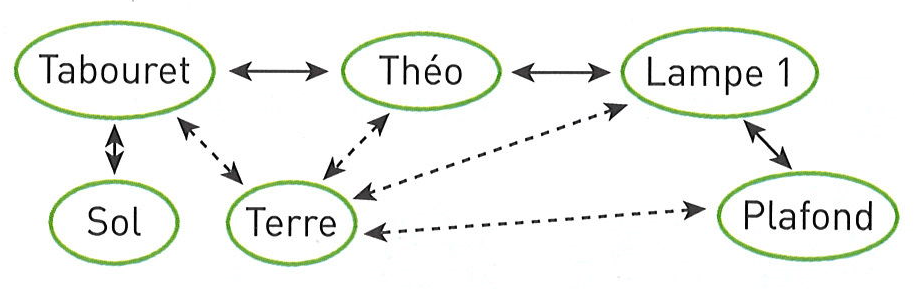
\includegraphics[scale=0.35]{doi2}
		\begin{solution}
			Théo est debout sur un tabouret et touche une lampe attachée au plafond.
		\end{solution}
		
	\end{questions}
\end{multicols}